\chapter{Feynman diagrams}
\section{a baby problem}
\begin{itemize}
	\item 考虑如下积分,
	\begin{equation} \label{3.1.1}
		Z(J) = \int_{- \infty}^{+ \infty} dq \, e^{- \frac{1}{2} m^2 q^2 - \frac{\lambda}{4!} q^4 + J q}
	\end{equation}
	
	\item \textbf{Schwinger's way:} 把 integrand 对 $\lambda$ 展开, 并将 $q$ 用 $\frac{\partial}{\partial J}$ 替代, 得到,
	\begin{align}
		Z(J) &= e^{- \frac{\lambda}{4!} (\frac{\partial}{\partial J})^4} \int_{- \infty}^{+ \infty} dq \, e^{- \frac{1}{2} m^2 q^2 + J q} \notag \\
		&= \sqrt{\frac{2 \pi}{m^2}} e^{- \frac{\lambda}{4!} (\frac{\partial}{\partial J})^4} e^{\frac{J^2}{2 m^2}} \label{3.1.2}
	\end{align}
	后面的计算中忽略 $Z(J = 0, \lambda = 0)$.
	
	\item 每个 vertex 带有 $- \lambda$, 每个 line 带有 $\frac{1}{m^2}$, 剩下的系数通过展开项算, 如下 (numerical factors 最好通过 Wick's way 算, 不过 baby problem 里 $q$ 无法区分, 所以不方便算, 先略了),
	
	\begin{figure}[H]
		\centering
		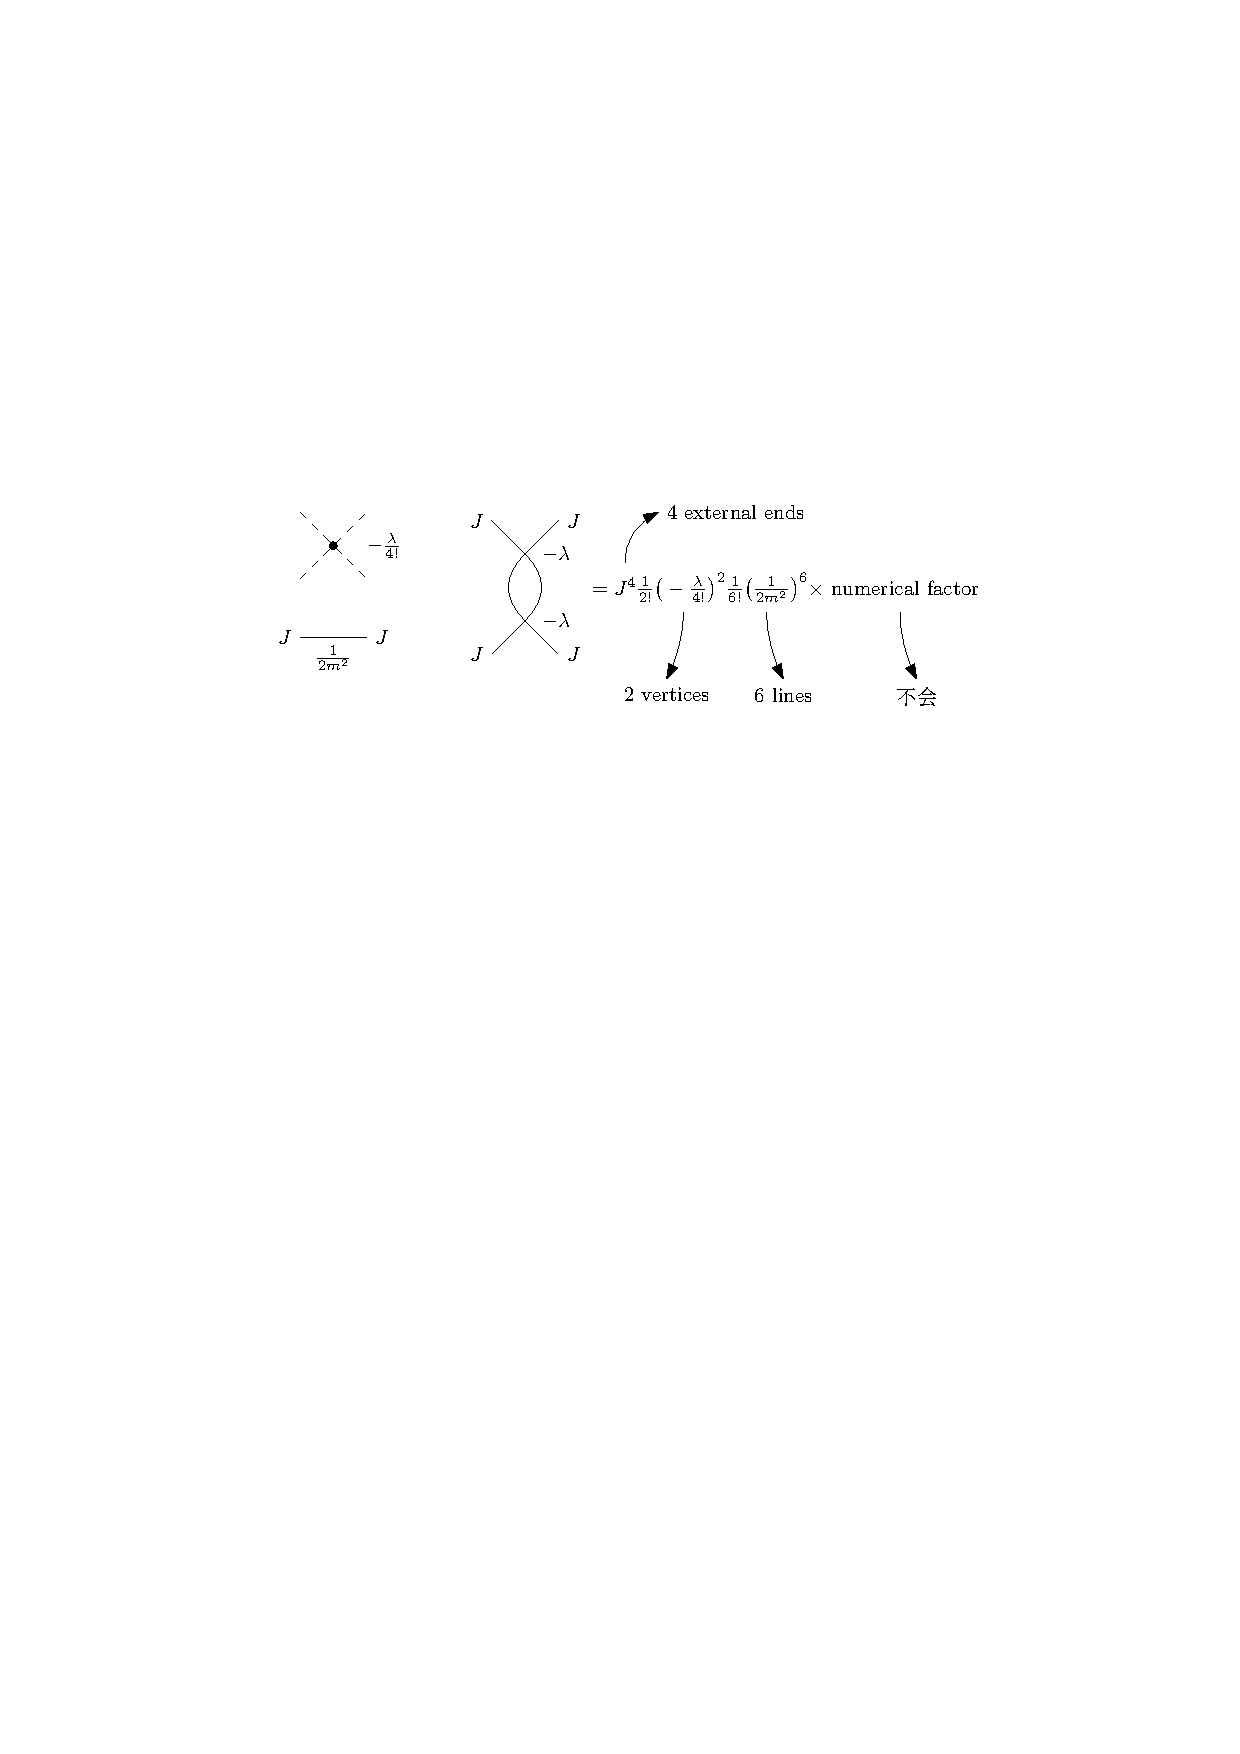
\includegraphics[scale=1]{figures/a baby problem - Feynman diagram.pdf}
	\end{figure}
	
	\begin{tcolorbox}[title=calculation:]
		在这里计算 $\lambda J^4$ 项,
		\begin{equation}
			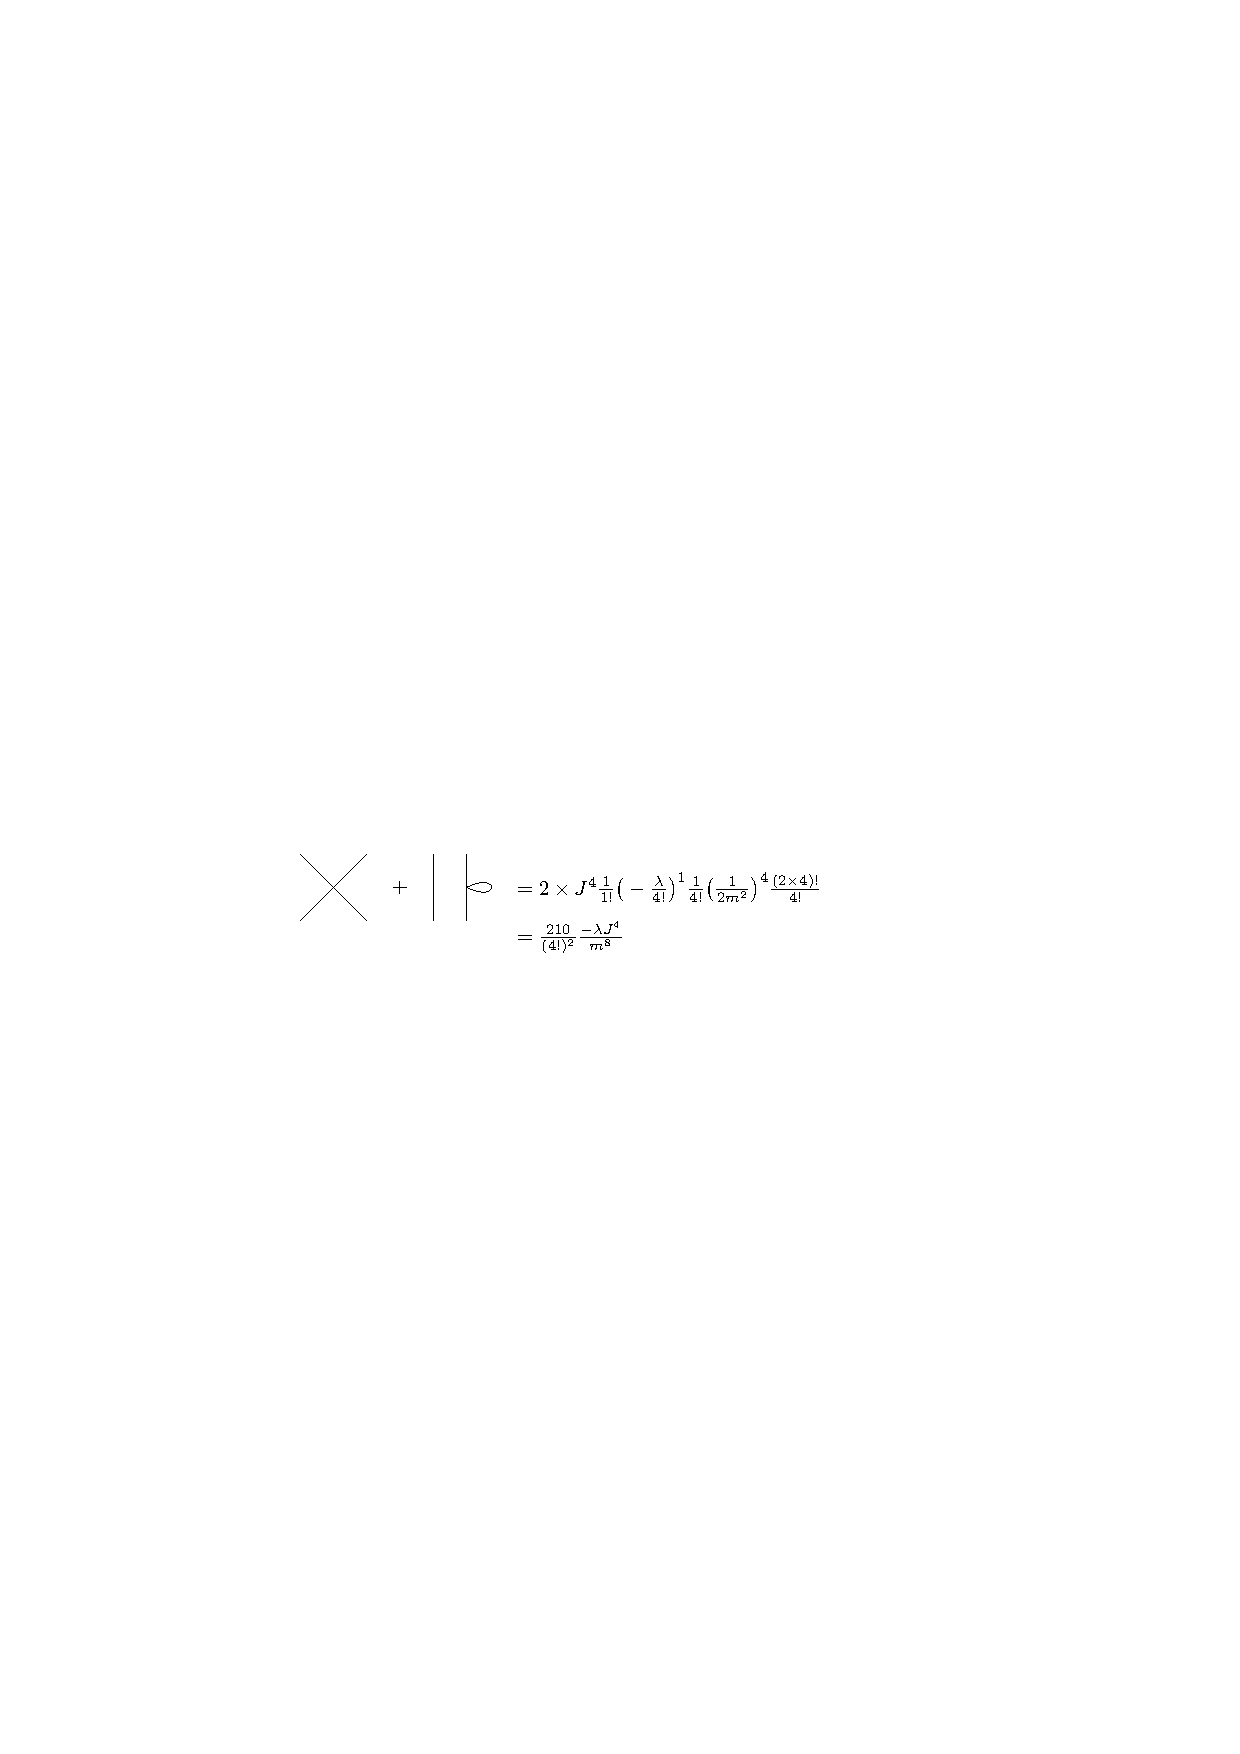
\includegraphics[scale=1]{figures/a baby problem - lambda J^4 terms.pdf}
		\end{equation}
		但是直接计算 \eqref{3.1.2} 的展开项, 得到的结果与 \eqref{3.1.5} 一样.
	\end{tcolorbox}
\end{itemize}

\subsection{Wick contraction and Green's functions}
\begin{itemize}
	\item 把积分 \eqref{3.1.1} 对 $J$ 展开,
	\begin{equation}
		Z(J) = \sum_{n = 0}^\infty \frac{1}{n!} J^n \underbrace{\int_{- \infty}^{+ \infty} dq \, e^{- \frac{1}{2} m^2 q^2 - \frac{\lambda}{4!} q^4} q^n}_{= Z(0, 0) G^{(n)}}
	\end{equation}
	其中 Green's function $G^{(n)}$ 对 $\lambda$ 展开后, 可以用 Wick contraction 计算 (见 \eqref{B.1.5}), 这就是 \textbf{Wick's way}.
	
	\begin{tcolorbox}[title=calculation:]
		计算 $\lambda J^4$ 项, 它来自 $G^{(4)}$ 对 $\lambda$ 展开的一阶项,
		\begin{align}
			- \frac{\lambda}{4!} \int dq \, e^{- \frac{1}{2} m^2 q^2} q^8 &= - \frac{\lambda}{4!} \braket{q^8} \notag \\
			&= - \frac{\lambda}{4!} \sum_{\text{Wick}} \Big( \frac{1}{m^2} \Big)^4 \notag \\
			&= - \frac{\lambda}{4!} \frac{7 \times 5 \times 3 \times 1}{m^8} \label{3.1.5}
		\end{align}
		所以 $\lambda J^4$ 项等于 $\frac{105}{(4!)^2} \frac{- \lambda J^4}{m^8}$.
	\end{tcolorbox}
\end{itemize}

\subsection{connected vs. disconnected}
\begin{itemize}
	\item 考虑,
	\begin{equation}
		Z(J, \lambda) = Z(J = 0, \lambda) e^{W(J, \lambda)}
	\end{equation}
	其中 $Z(J = 0, \lambda)$ 由 diagrams with no external source $J$ 组成, 而 $W(J, \lambda)$ 则由 connected diagrams 组成 \textcolor{red}{(?)}.
	
	\item 我们希望计算的是 $W$, 而不是 $Z$ \textcolor{red}{(?)}.
\end{itemize}

\section{a child problem}
\begin{itemize}
	\item 考虑如下积分,
	\begin{equation}
		Z(J) = \int dq_1 \cdots dq_N \, e^{- \frac{1}{2} q^T \cdot A \cdot q - \frac{\lambda}{4!} q^4 + J^T \cdot q}
	\end{equation}
	其中 $q^4 = \sum_i q_i^4$.
	
	\item \textbf{Schwinger's way:} 对 $\lambda$ 展开并把 $q$ 替换为 $\frac{\partial}{\partial J}$, 得到,
	\begin{equation}
		Z(J) = \sqrt{\frac{(2 \pi)^N}{\det A}} e^{- \frac{\lambda}{4!} (\frac{\partial}{\partial J})^4} e^{\frac{1}{2} J^T \cdot A^{- 1} \cdot J}
	\end{equation}
	其中 $\big( \frac{\partial}{\partial J} \big)^4 = \sum_i \big( \frac{\partial}{\partial J_i} \big)^4$.
\end{itemize}

\subsection{\texorpdfstring{$n$}{n}-point Green's function}
\begin{itemize}
	\item \textbf{Wick's way:} 对 $J$ 展开获得带 Green's function 的表达式,
	\begin{equation}
		Z(J) = \sum_{n = 0}^\infty \frac{1}{n!} \sum_{i_1 = 1}^N \cdots \sum_{i_n = 1}^N J_{i_1} \cdots J_{i_n} \underbrace{\int dq_1 \cdots dq_N \, e^{- \frac{1}{2} q^T \cdot A \cdot q - \frac{\lambda}{4!} q^4} q_{i_1} \cdots q_{i_n}}_{= Z(0, 0) G^{(n)}_{i_1 \cdots i_n}}
	\end{equation}
	其中 $G^{(n)}_{i_1 \cdots i_n}$ 称为 $n$-point Green's function.
	
	\begin{tcolorbox}[title=Taylor expansion:]
		多元函数的 Taylor 展开如下,
		\begin{align}
			f(x_1, \cdots, x_N) &= \sum_{n_1 = 0}^\infty \cdots \sum_{n_N = 0}^\infty \frac{x_1^{n_1}}{n_1 !} \cdots \frac{x_N^{n_N}}{n_N !} \frac{\partial^{n_1}}{\partial x_1^{n_1}} \cdots \frac{\partial^{n_N}}{\partial x_N^{n_N}} f(x = 0) \notag \\
			&= \sum_{n = 0}^\infty \frac{1}{n!} \sum_{i_1 = 1}^N \cdots \sum_{i_n = 1}^N x_{i_1} \cdots x_{i_n} \frac{\partial}{\partial x_{i_1}} \cdots \frac{\partial}{\partial x_{i_N}} f(x = 0)
		\end{align}
		这两种求和方法, $x_1^{n_1} \cdots x_N^{n_N}$ 项的 numerical factor 都等于,
		\begin{equation}
			\frac{1}{n!} \times \frac{n!}{n_1 ! \cdots n_N !} = \frac{1}{n_1 ! \cdots n_N !}
		\end{equation}
		其中 $n = n_1 + \cdots + n_N$.
	\end{tcolorbox}
	
	\item 在 $\lambda = 0$ 时, $2$-point Green's function 就是 propagator,
	\begin{align}
		G^{(2)}_{i j}(\lambda = 0) &= \frac{1}{Z(0, 0)} \int dq_1 \cdots dq_N \, e^{- \frac{1}{2} q^T \cdot A \cdot q} q_i q_j \notag \\
		&= \frac{\partial}{\partial J_i} \frac{\partial}{\partial J_j} e^{\frac{1}{2} J^T \cdot A^{- 1} \cdot J} \Big|_{J = 0} = A^{- 1}_{i j}
	\end{align}
	
	\item 来计算 $2, 3, 4$-point Green's functions,
	\begin{equation}
		\begin{dcases}
			G^{(2)}_{i j} = A^{- 1}_{i j} - \frac{\lambda}{4!} \sum_m (3 A^{- 1}_{m m} A^{- 1}_{m m} A^{- 1}_{i j} + 12 A^{- 1}_{m m} A^{- 1}_{m i} A^{- 1}_{m j}) + O(\lambda^2) \\
			G^{(3)}_{i j k} = 0 \\
			\begin{aligned}
				G^{(4)}_{i j k l} =& A^{- 1}_{i j} A^{- 1}_{k l} + A^{- 1}_{i k} A^{- 1}_{j l} + A^{- 1}_{i l} A^{- 1}_{j k} \\
				& - \frac{\lambda}{4!} \sum_m (A^{- 1}_{m m} A^{- 1}_{m m} A^{- 1}_{i j} A^{- 1}_{k l} + \cdots + 4! A^{- 1}_{i m} A^{- 1}_{j m} A^{- 1}_{k m} A^{- 1}_{l m}) + O(\lambda^2)
			\end{aligned}
		\end{dcases}
	\end{equation}
	
	\begin{tcolorbox}[title=calculation:]
		$2$-point Green's function 计算如下,
		\begin{align}
			G^{(2)}_{i j} &= \frac{1}{Z(0, 0)} \int dq_1 \cdots dq_N \, e^{- \frac{1}{2} q^T \cdot A \cdot q} \Big( 1 - \frac{\lambda}{4!} q^4 + O(\lambda^2) \Big) q_i q_j \notag \\
			&= A^{- 1}_{i j} - \frac{\lambda}{4!} \braket{q^4 q_i q_j} + O(\lambda^2) \notag \\
			&= A^{- 1}_{i j} - \frac{\lambda}{4!} \sum_m (3 A^{- 1}_{m m} A^{- 1}_{m m} A^{- 1}_{i j} + 12 A^{- 1}_{m m} A^{- 1}_{m i} A^{- 1}_{m j}) + O(\lambda^2)
		\end{align}
		$3$-point Green's function 计算如下,
		\begin{equation}
			G^{(32)}_{i j k} = \frac{1}{Z(0, 0)} \int dq_1 \cdots dq_N \, e^{- \frac{1}{2} q^T \cdot A \cdot q} \Big( 1 - \frac{\lambda}{4!} q^4 + O(\lambda^2) \Big) q_i q_j q_k = 0
		\end{equation}
		$4$-point Green's function 计算如下,
		\begin{align}
			G^{(4)}_{i j k l} &= \frac{1}{Z(0, 0)} \int dq_1 \cdots dq_N \, e^{- \frac{1}{2} q^T \cdot A \cdot q} \Big( 1 - \frac{\lambda}{4!} q^4 + O(\lambda^2) \Big) q_i q_j q_k q_l \notag \\
			&= A^{- 1}_{i j} A^{- 1}_{k l} + A^{- 1}_{i k} A^{- 1}_{j l} + A^{- 1}_{i l} A^{- 1}_{j k} - \frac{\lambda}{4!} \braket{q^4 q_i q_j q_k q_l} + O(\lambda^2)
		\end{align}
	\end{tcolorbox}
\end{itemize}

\section{perturbative field theory}
\begin{itemize}
	\item 做如下替换即可,
	\begin{equation}
		\begin{dcases}
			A \mapsto - i (\partial^2 - m^2) \\
			J \mapsto i J
		\end{dcases}
	\end{equation}
	
	\item \textbf{Schwinger's way:} $\phi^4$ theory 的路径积分,
	\begin{align}
		Z(J) &= \int D\phi \, e^{i \int d^d x \, (\frac{1}{2} \phi (\partial^2 - m^2) \phi - \frac{\lambda}{4!} \phi^4 + J(x) \phi(x))} \\
		&= Z(0, 0) e^{- i \frac{\lambda}{4!} \int d^d z \, (\frac{\delta}{i \delta J(z)})^4} e^{- \frac{i}{2} \int d^d x d^d y \, J(x) D(x - y) J(y)}
	\end{align}
	其中 $D(x - y)$ 是自由场的 propagator, 见 \eqref{1.2.1}.
	
	\item \textbf{Wick's way:} 同样, 对 $J$ 展开得到含 Green's functions 的表达式,
	\begin{equation}
		\frac{Z(J)}{Z(0, 0)} = \sum_{n = 0}^\infty \frac{i^n}{n!} \int d^d x_1 \cdots d^d x_n \, J(x_1) \cdots J(x_n) G^{(n)}(x_1, \cdots, x_n)
	\end{equation}
	其中,
	\begin{equation} \label{3.3.5}
		G^{(n)}(x_1, \cdots, x_n) = \frac{1}{Z(0, 0)} \int D\phi \, e^{i \int d^d x \, (\frac{1}{2} \phi (\partial^2 - m^2) \phi - \frac{\lambda}{4!} \phi^4)} \phi(x_1) \cdots \phi(x_n)
	\end{equation}
	有时 $Z(J)$ 被称为 generating functional, 因为它能生成 Green's functions.
\end{itemize}

\subsection{collision between particles}
\begin{itemize}
	\item 通过 Wick's way, 考虑 $J(x_1) J(x_2) J(x_3) J(x_4)$ 项, 实际上就是要计算 $G^{(4)}(x_1, x_2, x_3, x_4)$, 它的 0 阶项为,
	\begin{align}
		G^{(4)}(x_1, x_2, x_3, x_4, \lambda = 0) &= \frac{\delta}{i \delta J(x_1)} \frac{\delta}{i \delta J(x_2)} \frac{\delta}{i \delta J(x_3)} \frac{\delta}{i \delta J(x_4)} e^{- \frac{i}{2} \int d^d x d^d y \, J(x) D(x - y) J(y)} \notag \\
		&= - (D_{1 2} D_{3 4} + D_{1 3} D_{2 4} + D_{1 4} D_{2 3})
	\end{align}
	其中 $D_{i j}$ 是 $D(x_i - x_j)$ 的简写, 可见, 传播子实际上是 $(- i)^3 D = i D$.
	
	\item $G^{(4)}_{1 2 3 4}$ 的 1 阶项为,
	\begin{align}
		\text{1st order term} =& - \frac{i \lambda}{4!} \int d^d z \, \braket{\phi_1 \cdots \phi_4 \phi^4(z)} \notag \\
		=& - \frac{i \lambda}{4!} \int d^d z \, \frac{\delta}{i \delta J_1} \cdots \frac{\delta}{i \delta J_4} \Big( \frac{\delta}{i \delta J(z)} \Big)^4 e^{- \frac{i}{2} \int d^d x d^d y \, J(x) D(x - y) J(y)} \notag \\
		=& - \frac{i \lambda}{4!} \int d^d z \, \Big( 4! D_{1 z} D_{2 z} D_{3 z} D_{4 z} \notag \\
		& + 4 \times 3 D_{1 2} D_{3 z} D_{4 z} D_{z z} + \cdots + 3 D_{1 2} D_{3 4} D_{z z} D_{z z} + \cdots \Big)
	\end{align}
	其中各项分别对应如下 Feynman diagrams,
	
	\begin{figure}[H]
		\centering
		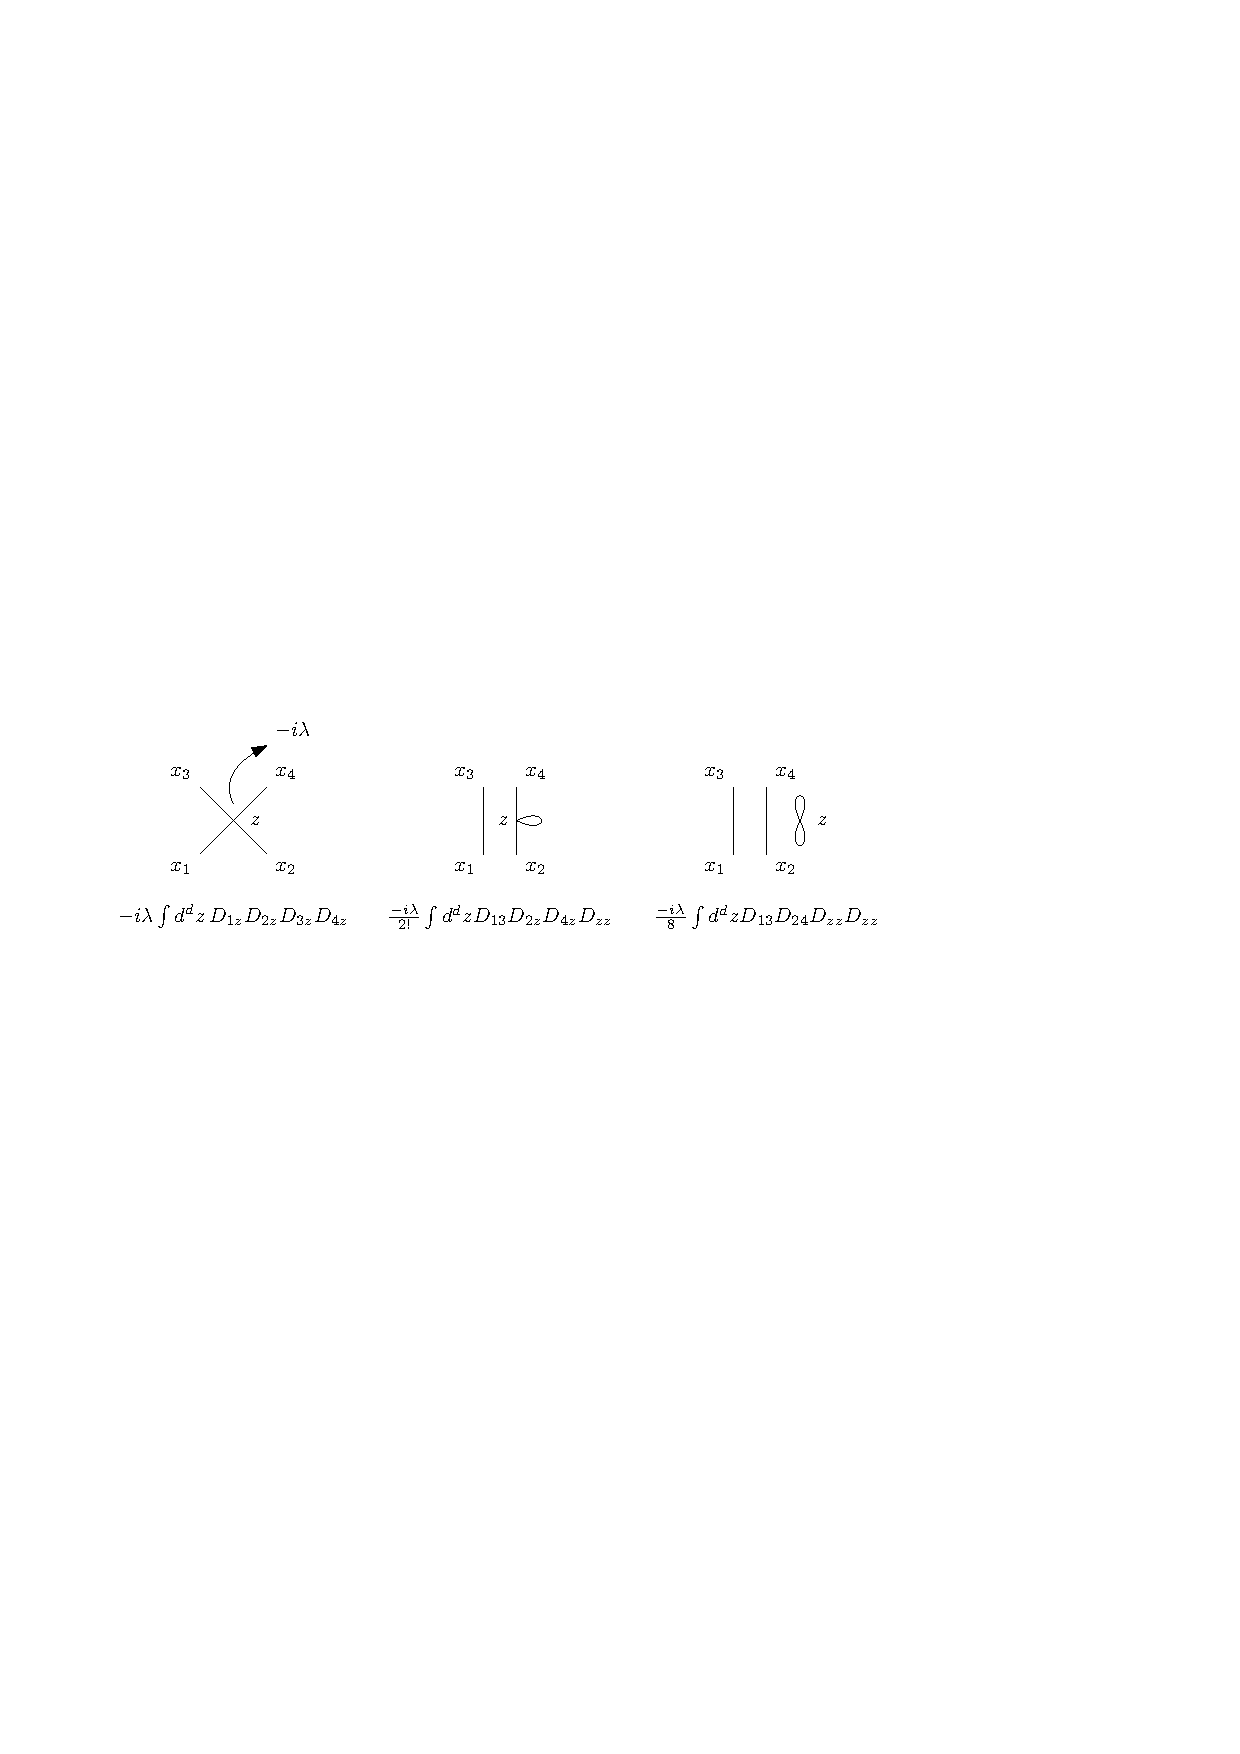
\includegraphics[scale=1]{figures/collision between particles - Feynman diagrams.pdf}
	\end{figure}
	
	其中 numerical factor 可以从 vertex 的四个 external end 的对称性得出.
	
	\item 再举一个例子,
	
	\begin{figure}[H]
		\centering
		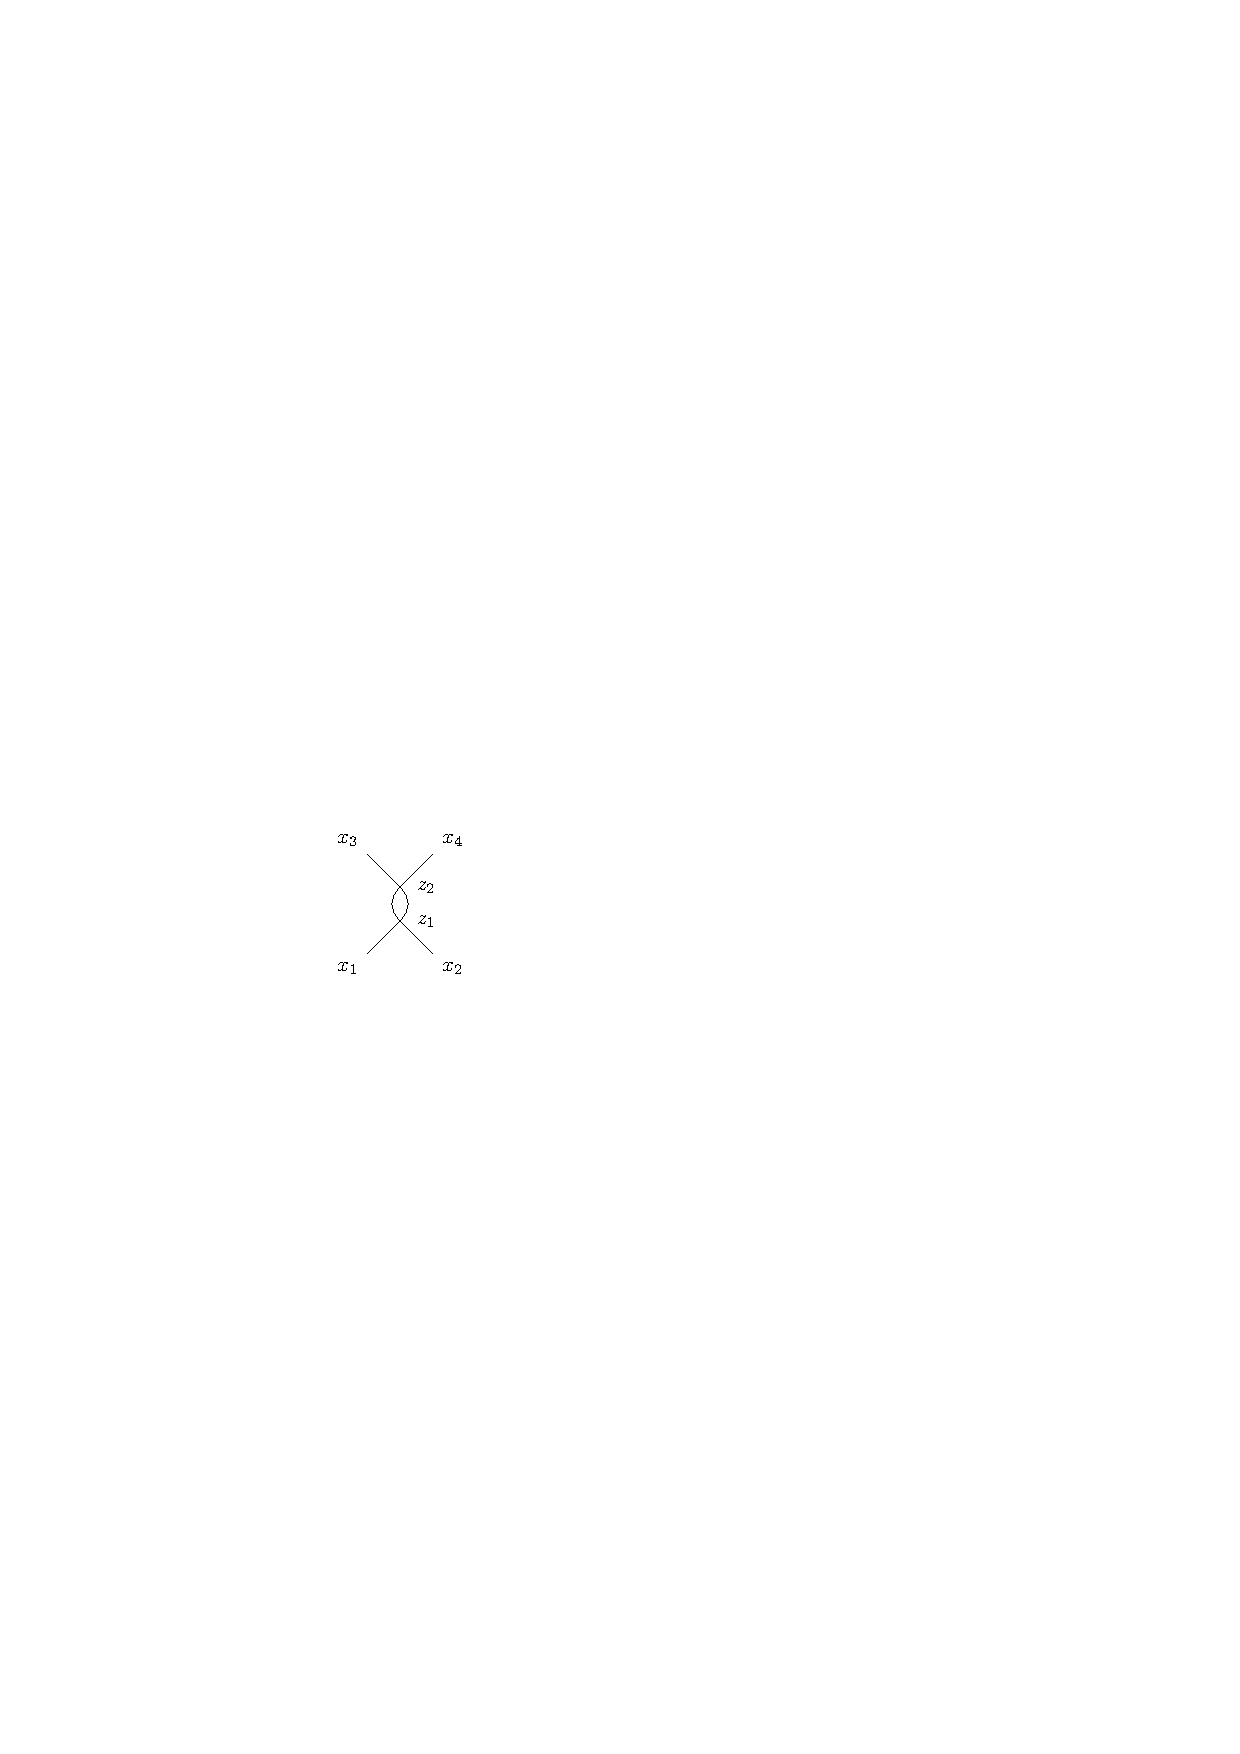
\includegraphics[scale=1]{figures/collision between particles - another Feynman diagram.pdf}
	\end{figure}
\end{itemize}

\subsection{in momentum space} \label{subsection 3.3.2}
\begin{itemize}
	\item 本 subsection 将 \eqref{3.3.5} 转换到 momentum space, 注意到 $\tilde{J}(k)$ 和 $\tilde{J}(- k)$ 并不独立, 所以 $\frac{\partial}{\partial i \tilde{J}}$ 不适用. 最方便的办法是直接对 position space 下的结果做 Fourier transformation,
	\begin{align}
		\tilde{G}^{(n)}(k_1, \cdots, k_n) &= \int d^d x_1 \cdots d^d x_n \, e^{- i (k_1 \cdot x_1 + \cdots)} G^{(n)}(x_1, \cdots, x_n) \notag \\
		&= \sum_{n = 0}^\infty \frac{1}{n!} \int d^d x_1 \cdots d^d x_n \, e^{- i (k_1 \cdot x_1 + \cdots)} \braket{\Big( - \frac{i \lambda}{4!} \int d^d z \, \phi_z^4 \Big)^n \phi_1 \cdots \phi_n}
	\end{align}
	\begin{itemize}
		\item propagator 的 Fourier transformation 是,
		\begin{equation}
			\tilde{D}_{p q} = \int d^d x d^d y \, e^{- i (p \cdot x + q \cdot y)} D(x - y) = \frac{(2 \pi)^d \delta^{(d)}(p + q)}{- p^2 - m^2 + i \epsilon}
		\end{equation}
		但似乎没有用.
	\end{itemize}
	
	\item $\tilde{G}^{(4)}(k_1, k_2, k_3, k_4)$ 的 1 阶项为,
	\begin{align}
		\text{1st order term} =& - \frac{i \lambda}{4!} \int d^d x_1 \cdots d^d x_4 \, e^{- i (k_1 \cdot x_1 + \cdots)} \int d^d z \, \braket{\phi_z^4 \phi_1 \cdots \phi_4}
	\end{align}
	考虑第 1 项,
	\begin{align}
		& - \frac{i \lambda}{4!} \int d^d x_1 \cdots d^d x_4 \, e^{- i (k_1 \cdot x_1 + \cdots)} \int d^d z \, 4! D_{1 z} \cdots D_{4 z} \notag \\
		=& - i \lambda \int d^d x_1 \cdots d^d x_4 d^d z \, e^{- i (k_1 \cdot x_1 + \cdots)} e^{i (p_1 \cdot (x_1 - z) + \cdots)} \prod_{i = 1}^4 \int \frac{d^d p_i}{(2 \pi)^d} \, \frac{1}{- p_i^2 - m^2 + i \epsilon} \notag \\
		=& - i \lambda \underbrace{\int d^d z \, e^{- i z \cdot (k_1 + \cdots + k_4)}}_{= (2 \pi)^d \delta^{(d)}(k_1 + \cdots + k_4)} \prod_{i = 1}^4 \frac{1}{- k_i^2 - m^2 + i \epsilon}
	\end{align}
	\begin{itemize}
		\item 出射粒子不一定 on-shell \textcolor{red}{(?)}.
	\end{itemize}
	
	\item 得到这些 Feynman diagrams,
	
	\begin{figure}[H]
		\centering
		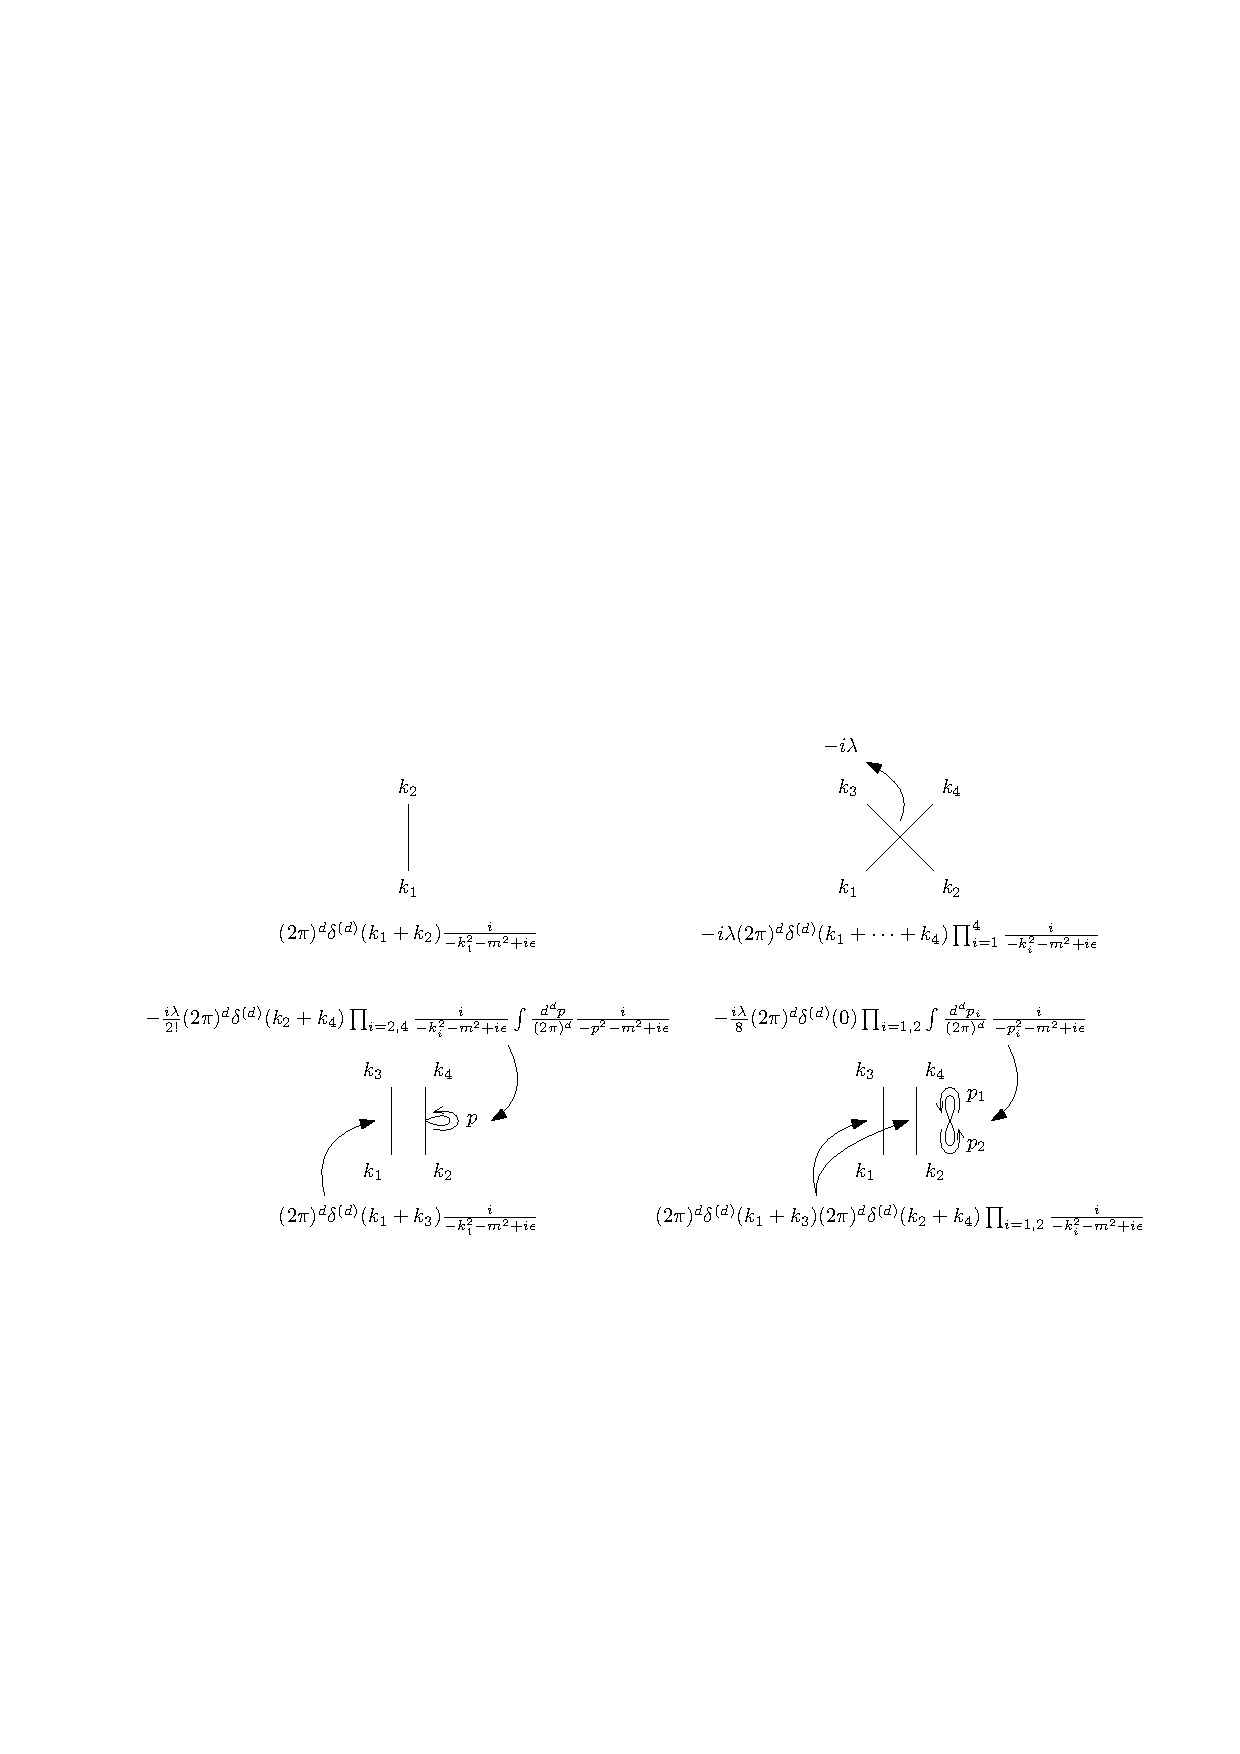
\includegraphics[scale=1]{figures/collision between particles - Feynman diagrams (in momentum space).pdf}
	\end{figure}
	
	\begin{tcolorbox}[title=calculation:]
		第 3 幅图的计算如下,
		\begin{align}
			& - \frac{i \lambda}{2!} \int d^d x_1 \cdots d^d x_4 \, e^{- i (k_1 \cdot x_1 + \cdots)} \int d^d z \, D_{1 3} D_{2 z} D_{4 z} D_{z z} \notag \\
			=& - \frac{i \lambda}{2!} \int d^d x_1 \cdots d^d x_4 d^d z \, e^{- i (k_1 \cdot x_1 + \cdots)} e^{i (p_1 \cdot (x_1 - x_3) + p_2 \cdot (x_2 - z) + p_4 \cdot (x_4 - z) + p_4 \cdot 0)} \notag \\
			& \prod_{i = 1}^4 \int \frac{d^d p_i}{(2 \pi)^d} \, \frac{1}{- p_i^2 - m^2 + i \epsilon} \notag \\
			=& - \frac{i \lambda}{2!} \int d^d z \, e^{- i z \cdot (p_2 + p_4)} \delta^{(d)}(p_1 - k_1) \delta^{(d)}(p_2 - k_2) \delta^{(d)}(p_1 + k_3) \delta^{(d)}(p_4 - k_4) \notag \\
			& \prod_{i = 1}^4 \int d^d p_i \frac{1}{- p_i^2 - m^2 + i \epsilon} \notag \\
			=& - \frac{i \lambda}{2!} (2 \pi)^d \delta^{(d)}(k_1 + k_3) \delta^{(d)}(k_2 + k_4) \prod_{i = 1, 2, 4} \frac{1}{- k_i^2 - m^2 + i \epsilon} \int \frac{d^d p}{- p^2 - m^2 + i \epsilon}
		\end{align}
		第 4 幅图的计算如下,
		\begin{align}
			& - \frac{i \lambda}{8} \int d^d x_1 \cdots d^d x_4 \, e^{- i (k_1 \cdot x_1 + \cdots)} \int d^d z \, D_{1 3} D_{2 4} D_{z z} D_{z z} \notag \\
			=& - \frac{i \lambda}{8} \int d^d x_1 \cdots d^d x_4 d^d z \, e^{- i (k_1 \cdot x_1 + \cdots)} e^{i (p_1 \cdot (x_1 - x_3) + p_2 \cdot (x_2 - x_4) + p_3 \cdot 0 + p_4 \cdot 0)} \notag \\
			& \prod_{i = 1}^4 \int \frac{d^d p_i}{(2 \pi)^d} \, \frac{1}{- p_i^2 - m^2 + i \epsilon} \notag \\
			=& - \frac{i \lambda}{8} \int d^d z \, \delta^{(d)}(p_1 - k_1) \delta^{(d)}(p_2 - k_2) \delta^{(d)}(p_1 + k_3) \delta^{(d)}(p_2 + k_4) \notag \\
			& \prod_{i = 1}^4 \int d^d p_i \, \frac{1}{- p_i^2 - m^2 + i \epsilon} \notag \\
			=& - \frac{i \lambda}{8} (2 \pi)^d \delta^{(d)}(0) \delta^{(d)}(k_1 + k_3) \delta^{(d)}(k_2 + k_4) \prod_{i = 1, 2} \frac{1}{- k_i^2 - m^2 + i \epsilon} \notag \\
			& \prod_{i = 1, 2} \int d^d p_i \, \frac{1}{- p_i^2 - m^2 + i \epsilon}
		\end{align}
	\end{tcolorbox}
	
	\item 再举一个例子 (略去了 $\prod_{i = 1}^6 \frac{i}{- k_i^2 - m^2 + i \epsilon}$),
	\begin{align}
		& 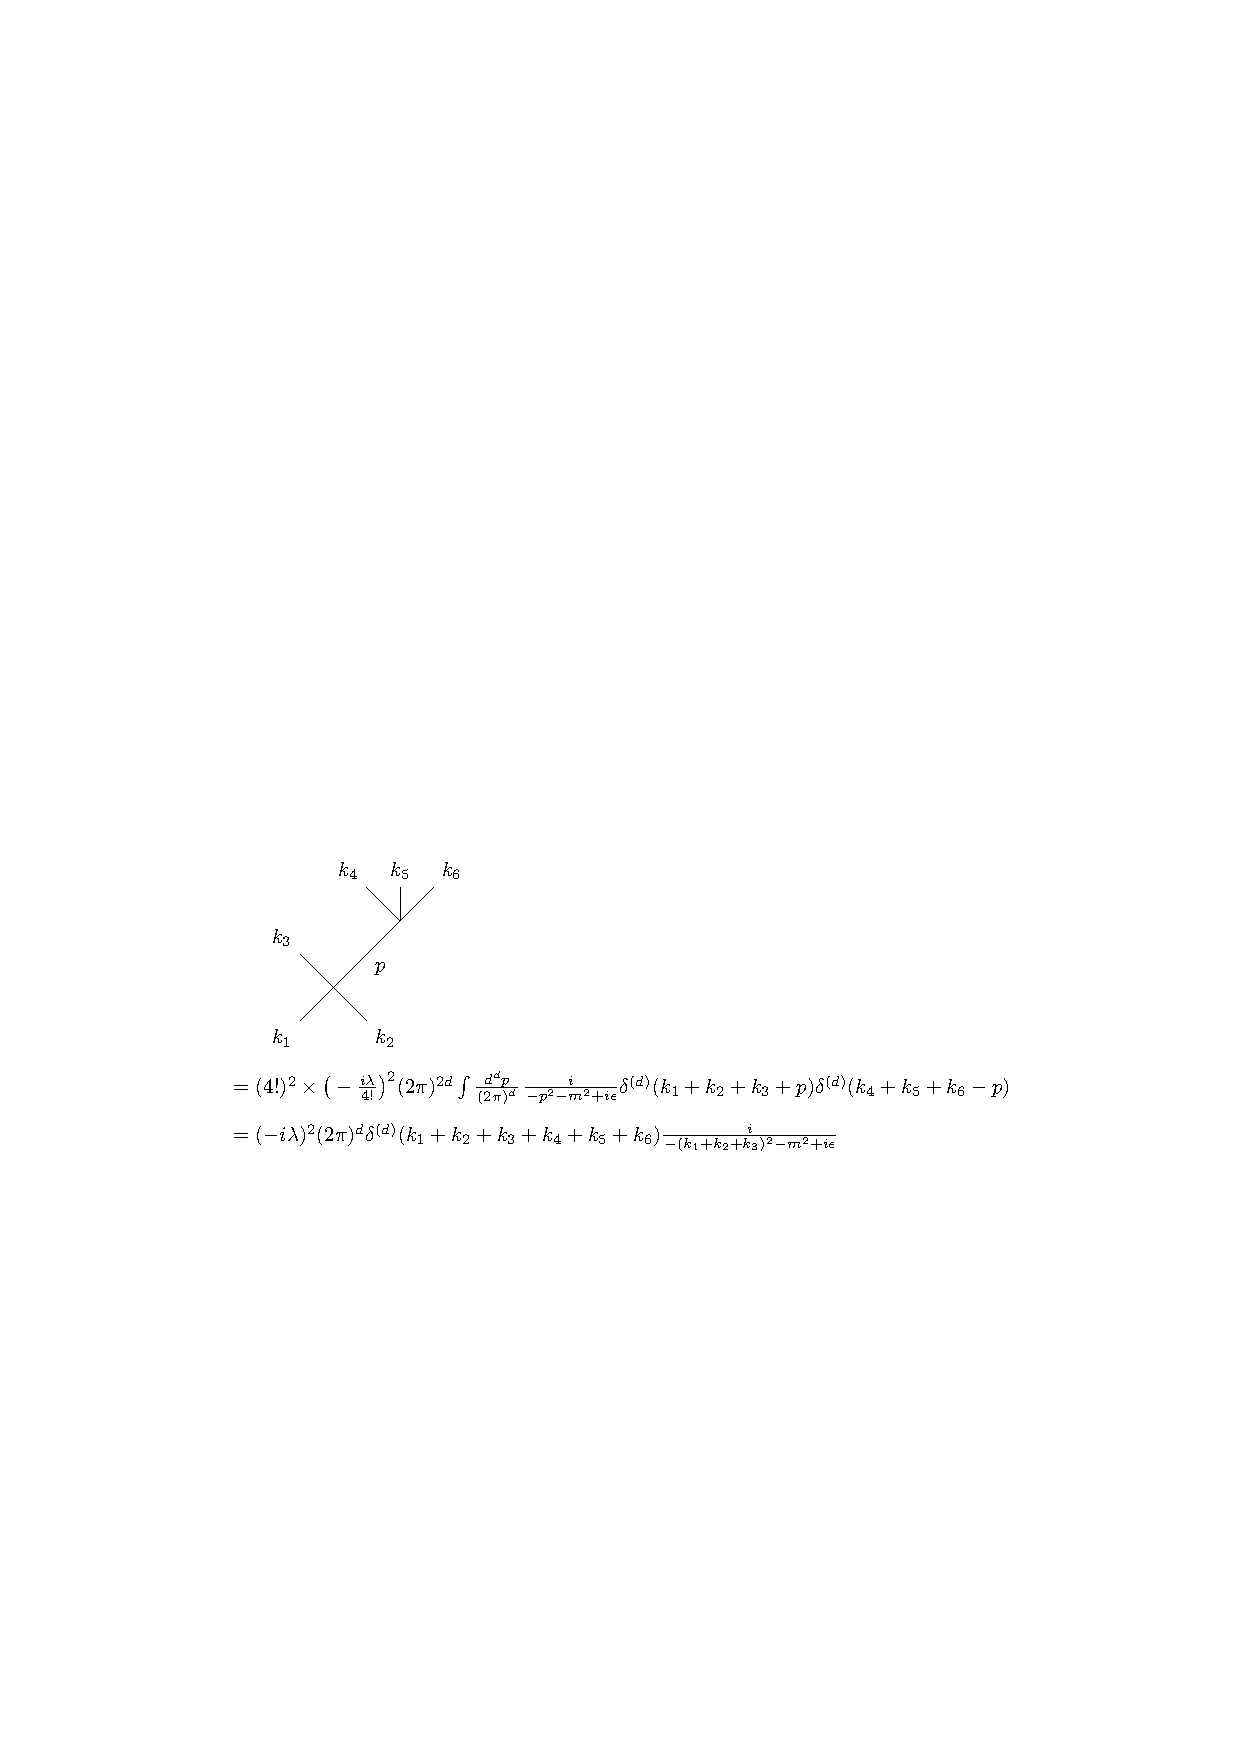
\includegraphics[scale=1]{figures/collision between particles - another Feynman diagram (in momentum space).pdf} \notag \\
		=& \frac{(4!)^2}{2!} \times \big( - \frac{i \lambda}{4!} \big)^2 (2 \pi)^{2 d} \int \frac{d^d p}{(2 \pi)^d} \, \frac{i}{- p^2 - m^2 + i \epsilon} \delta^{(d)}(k_1 + k_2 + k_3 + p) \delta^{(d)}(k_4 + k_5 + k_6 - p) \notag \\
		=& \frac{(- i \lambda)^2}{2} (2 \pi)^d \delta^{(d)}(k_1 + k_2 + k_3 + k_4 + k_5 + k_6) \frac{i}{- (k_1 + k_2 + k_3)^2 - m^2 + i \epsilon}
	\end{align}
\end{itemize}

\subsection{loops and a first look at divergence}
\begin{itemize}
	\item subsection \ref{subsection 3.3.2} 里的 loop diagrams 出现了如下积分,
	\begin{equation}
		\int \frac{d^d p}{(2 \pi)^d} \frac{i}{- p^2 - m^2 + i \epsilon} \overset{d = 4}{\sim} \int \frac{d^4 p}{p^2}
	\end{equation}
	积分发散.
	
	\item 再举一个例子 (略去了 $\prod_{i = 1}^4 \frac{i}{- k_i^2 - m^2 + i \epsilon}$),
	\begin{align}
		& 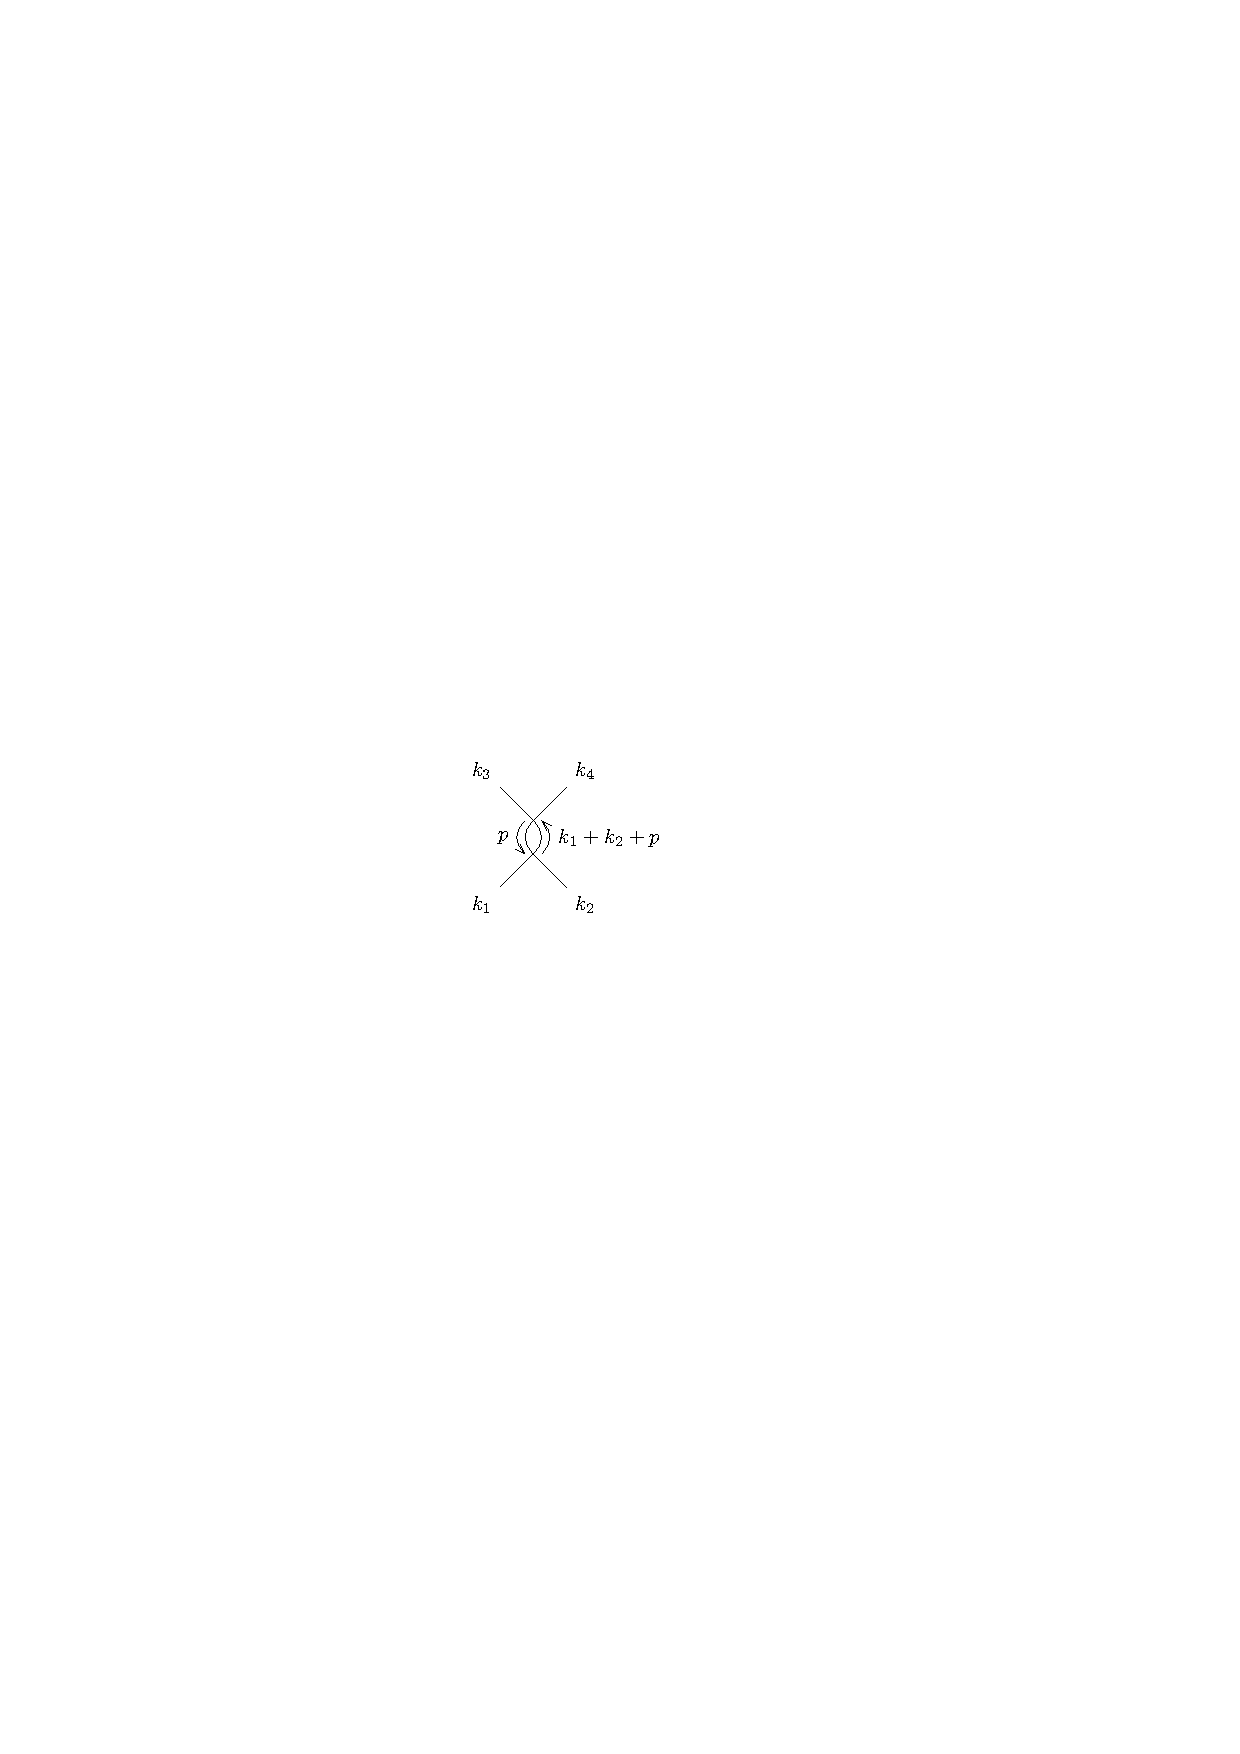
\includegraphics[scale=1]{figures/another loop diagram.pdf} \notag \\
		=& (4 \times 3)^2 \times 2 \times \frac{1}{2!} \times \Big( \frac{- i \lambda}{4!} \Big)^2 \int \frac{d^d p}{(2 \pi)^d} \frac{i}{- p^2 - m^2 + i \epsilon} \int \frac{d^d q}{(2 \pi)^d} \frac{i}{- q^2 - m^2 + i \epsilon} \notag \\
		& (2 \pi)^d \delta^{(d)}(k_1 + k_2 + p - q) (2 \pi)^d \delta^{(d)}(k_3 + k_4 - p + q) \notag \\
		=& \frac{(- i \lambda)^2}{4} (2 \pi)^d \delta^{(d)}(k_1 + k_2 + k_3 + k_4) \int \frac{d^d p}{(2 \pi)^d} \frac{i}{- p^2 - m^2 + i \epsilon} \frac{i}{- (k_1 + k_2 + p)^2 - m^2 + i \epsilon} \notag \\
		\overset{d = 4}{\sim} & \int \frac{d^4 p}{p^4}
	\end{align}
	同样, 积分发散.
\end{itemize}
